\documentclass[11pt]{article}

\usepackage[norsk]{babel}
\usepackage[utf8]{inputenc}
\usepackage{amsmath, amssymb, amsthm}
\usepackage{graphicx, float}
\usepackage{pstricks-add}


\author{Kjetil Kjeka}
\title{TTK4130 - Exercise 6}
\date{\today}


%Slik at matriser kan defineres med linjer
\makeatletter
\renewcommand*\env@matrix[1][*\c@MaxMatrixCols c]{%
  \hskip -\arraycolsep
  \let\@ifnextchar\new@ifnextchar
  \array{#1}}
\makeatother

\newcommand{\abs}[1]{|#1|} 


\begin{document}
\maketitle
\section*{Problem 1}
For the system
\begin{eqnarray*}
\dot{u} &=& u (v-3) \\
\dot{v} &=& c (2-u)
\end{eqnarray*}
And the ``energy like'' function
\[V = u - 2 \ln{u} + v - 3 \ln{v} \]
\subsection*{a}
\[\dot{V} = u(v-3) - \frac{2}{u} u(v-3) + v(2-u) - \frac{3}{v} v(2-u) \]
\[\dot{V} = uv - 3u - 2v + 6 + 2v -vu - 6 + 3u = 0 \]
We don't got any theorems for what happends when function which is not positive definite derivate is not negative definite.

\subsection*{b}
Simulation of the Lotka-Voltera system for 20 timeunits is given in Figure \ref{fig:LotkaVoltera}
\begin{figure}[h]
\centering
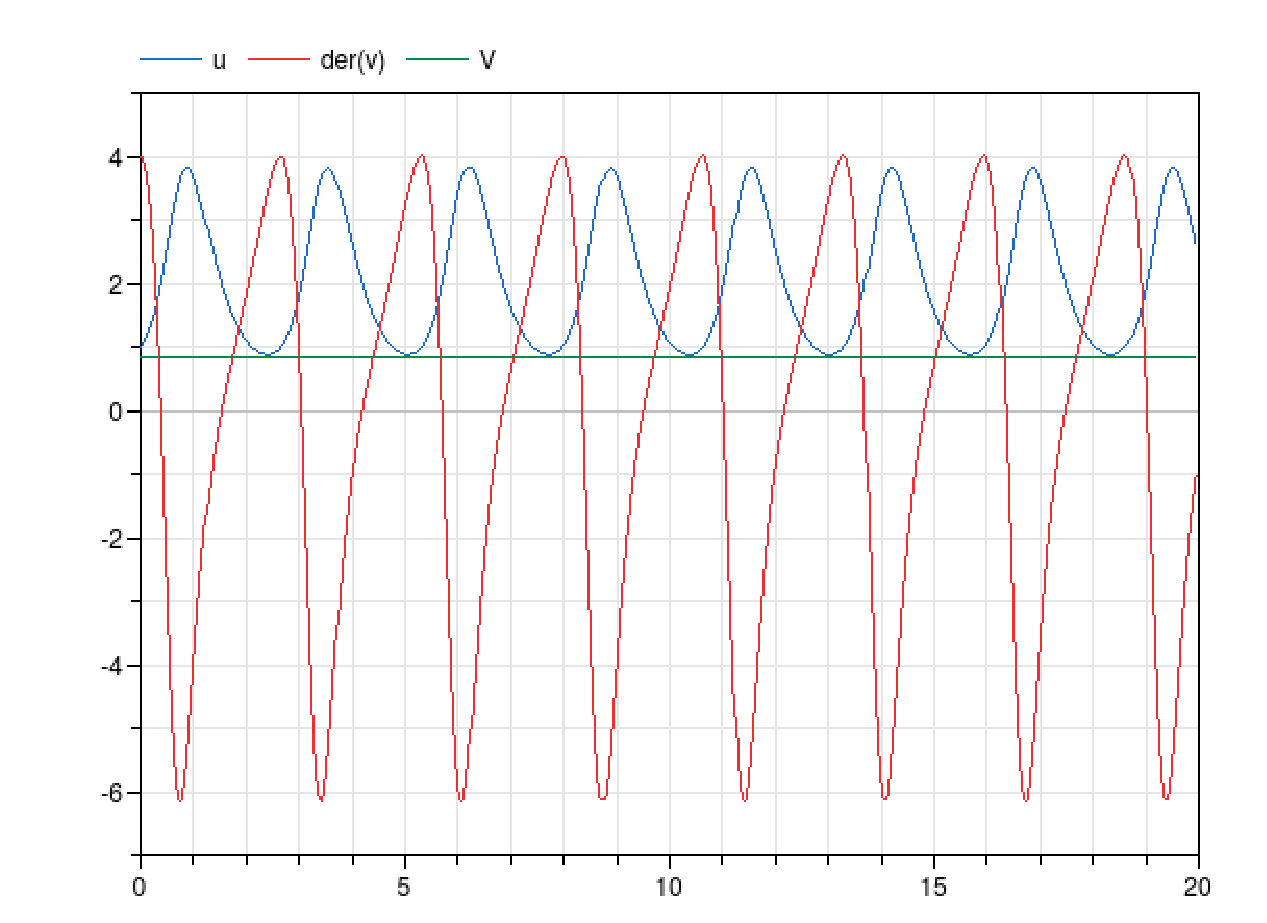
\includegraphics[width=.8\textwidth]{LotkaVoltera.eps}
\caption{Lotka-Voltera simulated for 20 time units}
\label{fig:LotkaVoltera}
\end{figure}

\subsection*{c}
The first order derivatives are:
\begin{eqnarray*}
\frac{df}{du} &=& \begin{bmatrix} v-3 \\ -v \end{bmatrix} \\
\frac{df}{dv} &=& \begin{bmatrix} u \\ 2-u \end{bmatrix} 
\end{eqnarray*}
Thus the linearization is:
\begin{eqnarray*}
\dot{u^*} &=&  2v \\
\dot{v^*} &=& -3u
\end{eqnarray*}
Which makes the eigenvalues
\[\lambda_{1,2} = \pm \sqrt{6} i \]
Which makes sense from Figure \ref{fig:LotkaVoltera} since the natural frequency $\omega$ is given by $\lambda = j\omega$ meaning $T = \frac{2 \pi}{\omega} = 2.6$

\subsection*{d}
The simulated models using the timestep $h = 0.05$ is given in Figure \ref{fig:LV_eeu} \ref{fig:LV_ieu} and \ref{fig:LV_imp}

\begin{figure}[h]
\centering
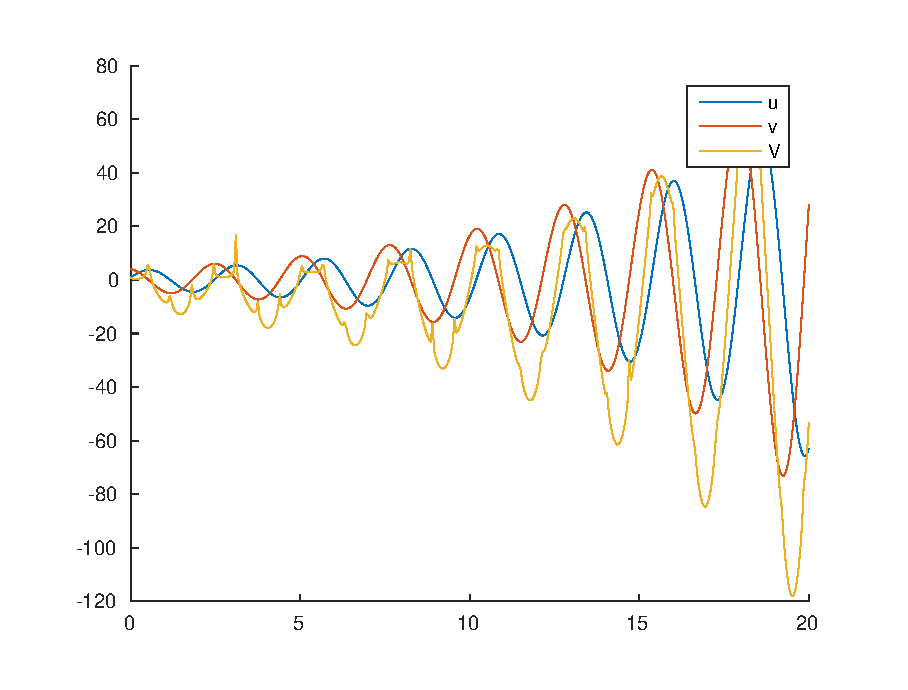
\includegraphics[width=.8\textwidth]{LV_eeu.eps}
\caption{Lotka-Voltera lineartization simulated for 20 time units with eulers method}
\label{fig:LV_eeu}
\end{figure}

\begin{figure}[h]
\centering
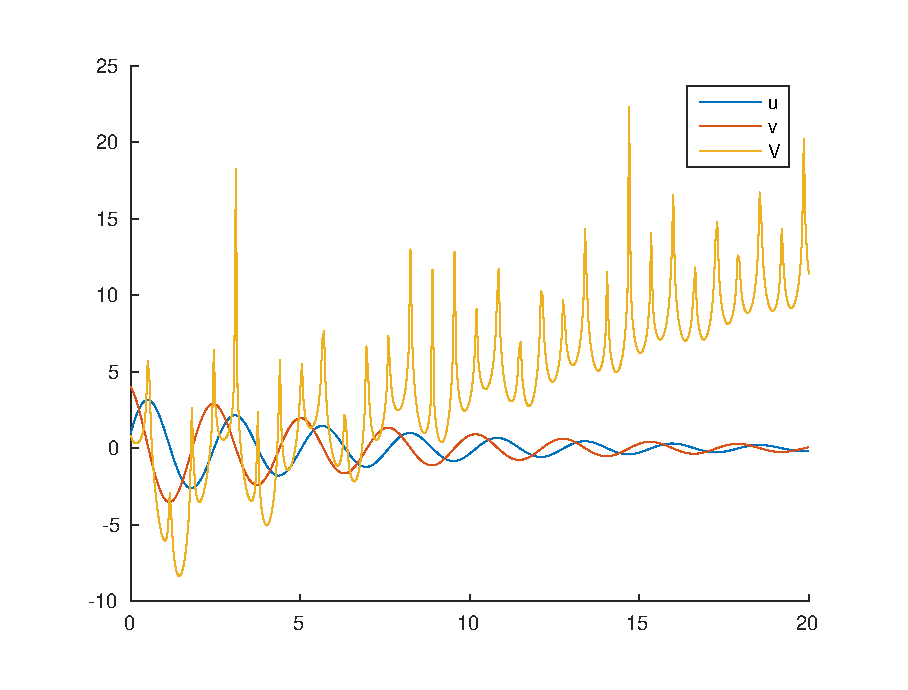
\includegraphics[width=.8\textwidth]{LV_ieu.eps}
\caption{Lotka-Voltera lineartization simulated for 20 time units with implicit eulers method}
\label{fig:LV_ieu}
\end{figure}

\begin{figure}[h]
\centering
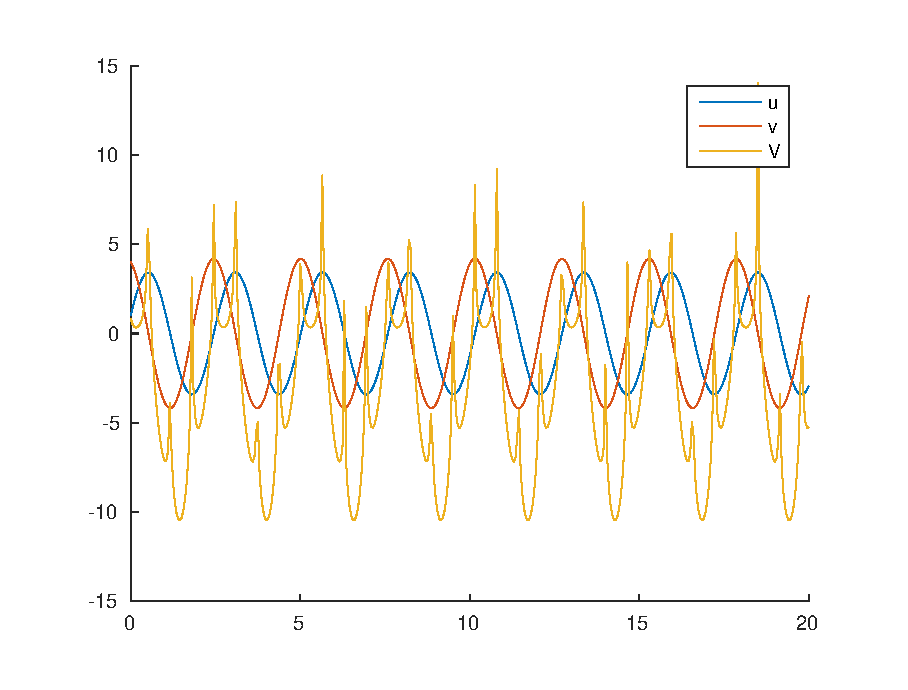
\includegraphics[width=.8\textwidth]{LV_imp.eps}
\caption{Lotka-Voltera lineartization simulated for 20 time units with implicit midpoint method}
\label{fig:LV_imp}
\end{figure}





\end{document}